% Created 2017-11-24 vie 17:15
% Intended LaTeX compiler: pdflatex
\documentclass[presentation]{beamer}
\usepackage[utf8]{inputenc}
\usepackage[T1]{fontenc}
\usepackage{graphicx}
\usepackage{grffile}
\usepackage{longtable}
\usepackage{wrapfig}
\usepackage{rotating}
\usepackage[normalem]{ulem}
\usepackage{amsmath}
\usepackage{textcomp}
\usepackage{amssymb}
\usepackage{capt-of}
\usepackage{hyperref}
\usepackage{minted}
\setminted[ipython]{frame=lines, fontsize=\tiny}
\setminted[python]{frame=lines, fontsize=\tiny}
\setminted[haskell]{frame=lines, fontsize=\tiny}
\usefonttheme[onlymath]{serif}
\usetheme{Boadilla}
\date{}
\title{GP - Rasmussen \& Williams - Ch. 2: Regression}
\hypersetup{
 pdfauthor={},
 pdftitle={GP - Rasmussen \& Williams - Ch. 2: Regression},
 pdfkeywords={},
 pdfsubject={},
 pdfcreator={Emacs 24.5.1 (Org mode 9.1.3)}, 
 pdflang={English}}
\begin{document}

\maketitle
\begin{frame}{Outline}
\tableofcontents
\end{frame}




\section{Regression}
\label{sec:orge261175}
\subsection{Sampling from prior}
\label{sec:org7e8b7e8}
\begin{frame}[label={sec:org0f401ca}]{GP prior}
\begin{eqnarray} \label{eg:GP}
k({x},{y}) & = & \mathrm{exp}( -\tfrac{1}{2}|{x}-{y}|^2) \\
\mathbf{f} & \sim & \mathcal{N}(\mathbf{0}, K(\mathbf{x}, \mathbf{x}))
\end{eqnarray}
\end{frame}


\begin{frame}[fragile,label={sec:orgce67762}]{Python code}
 \begin{minted}[]{ipython}
import numpy as np

def rbf(length_scale):
    def k(x,y):
        if len(x.shape)==1:
            d = 1
        else:
            d  = x.shape[1]
        lx = x.shape[0]
        ly = y.shape[0]
        dists =  np.sum(((x.T.reshape([d,lx,1]) -  y.T.reshape([d,1,ly]))/length_scale)**2,0)
        return np.exp(-.5 * dists)
    return k

def genSamplesSimple(x, k):
    n = x.shape[0]
    return np.random.multivariate_normal(np.zeros(n), k(x,x) + np.eye(n)*1e-8)

# def gesnSamplePostSimple(y,x,k,X):

# def gesnSamplePostSimple(y,x,k,X):
\end{minted}

\begin{minted}[]{python}
import matplotlib.pyplot as plt
plt.figure()
x = np.linspace(-5,5,150)
k = rbf(1)
for i in range(3): plt.plot(x, genSamplesSimple(x,k));
\end{minted}
\end{frame}


\begin{frame}[label={sec:orge696b02}]{Random functions in 1D}
\begin{center}
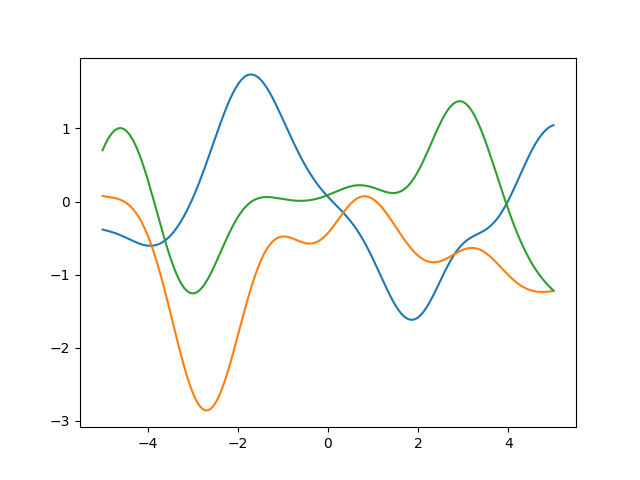
\includegraphics[width=.9\linewidth]{images/fig01.png}
\end{center}
\end{frame}


\begin{frame}[fragile,label={sec:org45154ca}]{Different length scales}
 \begin{columns}
\begin{column}{0.45\columnwidth}
\begin{minted}[]{python}
scales = [0.2, 1, 5]
for i in scales:
  plt.plot(x, genSamplesSimple(x,rbf(i)))
plt.legend(scales);
\end{minted}
\end{column}


\begin{column}{0.45\columnwidth}
\begin{center}
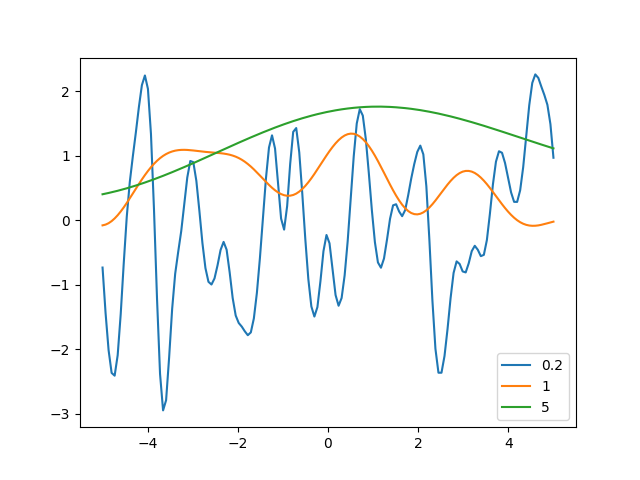
\includegraphics[width=.9\linewidth]{images/fig02.png}
\end{center}
\end{column}
\end{columns}
\end{frame}

\begin{frame}[fragile,label={sec:org531b380}]{Two dimensions}
 \begin{columns}
\begin{column}{0.45\columnwidth}
\begin{minted}[]{python}
x = np.linspace(5,-5,50)
xx, yy = np.meshgrid(x, x)
xy = np.concatenate(
       [xx.reshape([1,-1]),yy.reshape([1,-1])]).T
z = genSamplesSimple(xy, rbf(2)).reshape([50,50])
\end{minted}

\begin{minted}[]{python}
fig = plt.figure()
ax = fig.gca(projection='3d')
ax.plot_surface(xx, yy, z, rstride=8, 
                cstride=8, alpha=0.3)
cset = ax.contour(xx, yy, z, zdir='z',
                  offset=-2.5, cmap=cm.coolwarm)
cset = ax.contour(xx, yy, z, zdir='x', 
                  offset=-5, cmap=cm.coolwarm)
cset = ax.contour(xx, yy, z, zdir='y', 
                  offset=5, cmap=cm.coolwarm)

ax.set_xlabel('X')
ax.set_xlim(-5, 5)
ax.set_ylabel('Y')
ax.set_ylim(-5, 5)
ax.set_zlabel('Z')
ax.set_zlim(-2.5, 2.5)
\end{minted}
\end{column}

\begin{column}{0.6\columnwidth}
\begin{center}
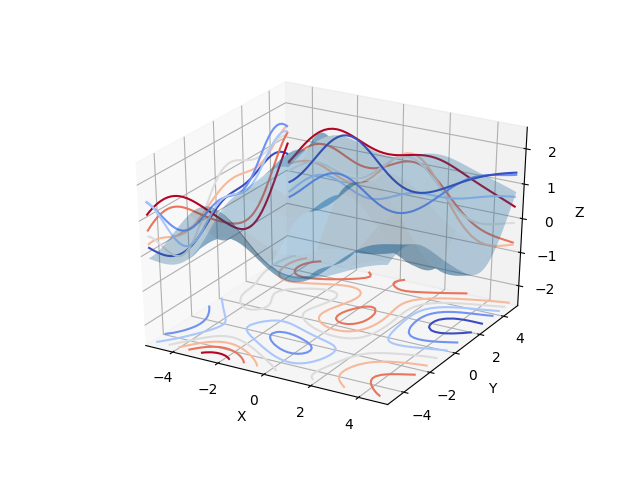
\includegraphics[width=.9\linewidth]{images/fig03.png}
\end{center}
\end{column}
\end{columns}
\end{frame}



\section{Exploration and classical hypothesis testing}
\label{sec:org868e051}
\subsection{Image noise and artifacts}
\label{sec:org5c6e92d}
\end{document}
